\documentclass[11pt]{amsart}
\usepackage{geometry}                % See geometry.pdf to learn the layout options. There are lots.
\geometry{letterpaper}                   % ... or a4paper or a5paper or ... 
%\geometry{landscape}                % Activate for for rotated page geometry
\usepackage[parfill]{parskip}    % Activate to begin paragraphs with an empty line rather than an indent
\usepackage{graphicx}
\usepackage{amssymb}
\usepackage{epstopdf}
\usepackage{amsmath}
\DeclareGraphicsRule{.tif}{png}{.png}{`convert #1 `dirname #1`/`basename #1 .tif`.png}

\title{Numerical Methods\\[0.1in]
	ECSE 543 - Assignment 2}
\author{Mido Assran - 260505216}
\date{\today}

\begin{document}
\maketitle

\section*{Question 1}
\vspace*{-0.2in}
\noindent\rule{\textwidth}{0.4pt}

The goal is to find the disjoint local \textbf{S}-matrix for each finite element triangle, and subsequently find the global conjoint \textbf{S}-matrix for the finite difference mesh composed of the triangular finite elements.

\begin{figure}[h]
    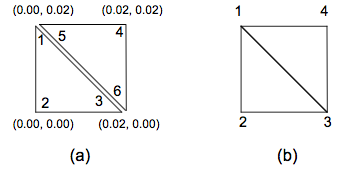
\includegraphics[width=0.6\textwidth]{assets/question_1.png}
    \caption{a) Disjoint finite elements with local numbering and vertex coordinates $(x,y)$ in meters b) Conjoint finite element mesh with global numbering}
    \label{fig:q1_mesh}
\end{figure}

The first step to finding the disjoint local \textbf{S}-matrix of each finite element triangle is to find the potentials in the elements. We take the potential, $U$, to vary linearly over the $(x,y)$ plane - note that the assumption of a linearly varying potential within the triangular element is equivalent to assuming that the electric field is uniform within the element (this is a good assumption in parallel-plate conductor type settings). Equation (\ref{eq:q1_potential}) shows the general linear relationship for the potential - constants $a$, $b$, and $c$ are to be determined.

\begin{equation}
	\label{eq:q1_potential}
	U = a + bx + cy
\end{equation}

Denoting the potentials at the vertices by $U_v$, where v is the vertex number set by the local ordering, we can solve the linear system of equations shown in equation (\ref{eq:q1_constants}) for the constants $a$, $b$, and $c$ where the potential at local vertex $v$ has coordinates given by $(x_v,y_v)$.

\begin{equation}
	\label{eq:q1_constants}
        \begin{bmatrix}
            U_1\\
            U_2\\
            U_3
        \end{bmatrix}
        =
        \begin{bmatrix}
            1 & x_1 & y_1\\ 
            1 & x_2 & y_2\\ 
            1 & x_3 & y_3 
        \end{bmatrix} 
        \begin{bmatrix}
            a\\
            b\\
            c
        \end{bmatrix}
\end{equation}

To solve for the constants we have the closed form relationship shown in equation (\ref{eq:q1_constants_closed_form}), where $adj$ is used to denote the adjugate of the matrix (found by taking the transpose of its cofactor matrix), and $det$ its determinant.

\begin{equation}
	\label{eq:q1_constants_closed_form}
        \begin{bmatrix}
            a\\
            b\\
            c
        \end{bmatrix}
        =
        \frac{
        	   adj
            \begin{bmatrix}
                1 & x_1 & y_1\\ 
                1 & x_2 & y_2\\ 
                1 & x_3 & y_3 
            \end{bmatrix}
            }{
            det
            \begin{bmatrix}
                1 & x_1 & y_1\\ 
                1 & x_2 & y_2\\ 
                1 & x_3 & y_3 
            \end{bmatrix}
        }
         \begin{bmatrix}
            U_1\\
            U_2\\
            U_3
        \end{bmatrix}
\end{equation}

The result of equation (\ref{eq:q1_constants_closed_form}) gives us the constants in terms of the vertex potentials as shown in equation (\ref{eq:q1_solved_cosntants}), where $A_e$ is used to denote the area of the triangular finite element $e$.

\begin{equation}
	\label{eq:q1_solved_cosntants}
        \begin{bmatrix}
            a\\
            b\\
            c
        \end{bmatrix}
        =
        \frac{
            \begin{bmatrix}
                (x_2y_3 - x_3y_2) & (x_3y_1 - x_1y_3) & (x_1y_2 - x_2y_1)\\ 
                (y_2 - y_3) & (y_3 - y_1) & (y_1 - y_2)\\ 
                (x_3 - x_2) & (x_1 - x_3) & (x_2 - x_1) 
            \end{bmatrix}
            }{
            2A_e
        	    }
         \begin{bmatrix}
            U_1\\
            U_2\\
            U_3
        \end{bmatrix}
\end{equation}

Since the potential in equation (\ref{eq:q1_potential}) can be written as 
$$ U =  
        \begin{bmatrix}
            1 & x & y
        \end{bmatrix}
	\begin{bmatrix}
            a\\
            b\\
            c
        \end{bmatrix}
$$

then we can directly substitute equation (\ref{eq:q1_solved_cosntants}) into the above representation and rewrite the potential as: $$ U = \sum^{3}_{i=1} \alpha_i(x,y) U_i$$

where the $\alpha_i(x,y)$ (also known as the linear interpolation functions) are given by equations (\ref{eq:q1_interpolation_functions_1}), (\ref{eq:q1_interpolation_functions_2}), and (\ref{eq:q1_interpolation_functions_3}),

\begin{equation}
    \label{eq:q1_interpolation_functions_1}
    \alpha_1 = \frac{1}{2A_e}[(x_2y_3 - x_3y_2) + (y_2 - y_3)x + (x_3 - x_2)y]
\end{equation}
\begin{equation}
    \label{eq:q1_interpolation_functions_2}
    \alpha_1 = \frac{1}{2A_e}[(x_3y_1 - x_1y_3) + (y_3 - y_1)x + (x_1 - x_3)y]
\end{equation}
\begin{equation}
    \label{eq:q1_interpolation_functions_3}
    \alpha_1 = \frac{1}{2A_e}[(x_1y_2 - x_2y_1) + (y_1 - y_2)x + (x_2 - x_1)y]
\end{equation}

and $A_e$ is given by equation (\ref{eq:q1_area}).

\begin{equation}
    \label{eq:q1_area}
    A_e = \frac{1}{2}[(x_2y_3 - x_3y_2) + (x_3y_1 - x_1y_3) + (x_1y_2 - x_2y_1)]
\end{equation}


The energy in each finite element is given by equation (\ref{eq:q1_energy}), where $W^{(e)}$ is the energy per unit length associated with finite element $e$, $U$ is the potential - which in general will vary with coordinates $(x,y)$ as was already established, and the integral is swept over $A_e$, which is the area occupied by element $e$. \footnotesize{*Note that there the permittivity of the medium is neglected in the equation}.
\begin{equation}
	\label{eq:q1_energy}
	W^{(e)} = \frac{1}{2} \int_{A_e}| \nabla U|^2 dS
\end{equation}

Equations (\ref{eq:q1_energy_2}), and (\ref{eq:q1_energy_3}) are derived by just making a simple substitution for $U$ in equation (\ref{eq:q1_energy}) using the derived series representation in terms of the interpolation functions and vertex potentials.

\begin{equation}
	\label{eq:q1_energy_2}
	W^{(e)} = \frac{1}{2}\sum^{3}_{i=1}\sum^{3}_{j=1}U_{i}\left[ \int_{A_e} \nabla \alpha_i \bullet \nabla \alpha_j dS \right]U_{j}
\end{equation}
\begin{equation}
	\label{eq:q1_energy_3}
	W^{(e)} = \frac{1}{2} U^T S^{(e)} U
\end{equation}

Finally we are able to determine the local $S^{(e)}$ depicted in equation (\ref{eq:q1_energy_3}), whose entries are given by equation (\ref{eq:q1_local_s}).

\begin{equation}
	\label{eq:q1_local_s}
	S^{(e)}_{(i,j)} = \int_{A_e} \nabla \alpha_i \bullet \nabla \alpha_j dS
\end{equation}

Therefore we have:

\begin{equation}
	\label{eq:q1_local_s11}
	S^{(e)}_{(1,1)} = \frac{1}{4A}[(y_2-y_3)^2 + (x_3 - x_2)^2]
\end{equation}
\begin{equation}
	\label{eq:q1_local_s12}
	S^{(e)}_{(1,2)} = \frac{1}{4A}[(y_2-y_3)(y_3 - y_1) + (x_3 - x_2)(x_1 - x_3)]
\end{equation}
\begin{equation}
	\label{eq:q1_local_s13}
	S^{(e)}_{(1,3)} = \frac{1}{4A}[(y_2-y_3)(y_1 - y_2) + (x_3 - x_2)(x_2 - x_1)]
\end{equation}
\begin{equation}
	\label{eq:q1_local_s22}
	S^{(e)}_{(2,2)} = \frac{1}{4A}[(y_3 - y_1)^2 + (x_1 - x_3)^2]
\end{equation}
\begin{equation}
	\label{eq:q1_local_s23}
	S^{(e)}_{(2,3)} = \frac{1}{4A}[(y_3 - y_1)(y_1 - y_2) + (x_1 - x_3)(x_2 - x_1)]
\end{equation}
\begin{equation}
	\label{eq:q1_local_s33}
	S^{(e)}_{(3,3)} = \frac{1}{4A}[(y_1 - y_2)^2 + (x_2 - x_1)^2]
\end{equation}
\begin{equation}
	\label{eq:q1_local_s_symmetry}
	S^{(e)}_{(1,2)} = S^{(e)}_{(2,1)}, \quad S^{(e)}_{(3,1)} = S^{(e)}_{(1,3)}, \quad S^{(e)}_{(3,2)} = S^{(e)}_{(2,3)}
\end{equation}

Letting $S^{(L)}$ represent the disjoint matrix for the lower triangular element in Figure \ref{fig:q1_mesh}.a, and $S^{(U)}$ represent the disjoint matrix for the upper triangular element in Figure \ref{fig:q1_mesh}.b, we can apply some \textit{plug-and-chug} to solve for the matrix entries where the local numberings relative to the derived equations are created in a counterclockwise fashion. The coordinates for the vertices in each element are:\\

\begin{center}
    \begin{tabular}{ c c } 
    $S^{(L)}$ & \\
    \hline
     $(x1,y1):$ & $(0,00, 0.02)$ \\ 
     $(x2,y2):$ & $(0.00, 0.00)$ \\ 
     $(x3,y3):$ & $(0.02, 0.00)$ \\[0.2in]
     $S^{(U)}$ & \\
     \hline
     $(x1,y1):$ & $(0.02, 0.02)$ \\ 
     $(x2,y2):$ & $(0.00, 0.02)$ \\ 
     $(x3,y3):$ & $(0.02, 0.00)$ \\ 

\end{tabular}
\end{center}

We have $A_e = \frac{1}{2}[(0.02 \cdot 0.02)] = 0.0002$, which is identical for $e = L$ and $e = U$.

$$
	S^{(L)}_{(1,1)} = \frac{1}{4(0.0002)}[(0.02)^2]
$$$$
	S^{(L)}_{(1,2)} = \frac{1}{4(0.0002)}[(0.02)(-0.02)]
$$$$
	S^{(L)}_{(1,3)} = \frac{1}{4(0.0002)}[0]
$$$$
	S^{(L)}_{(2,2)} = \frac{1}{4(0.0002)}[(-0.02)^2 + (-0.02)^2]
$$$$
	S^{(L)}_{(2,3)} = \frac{1}{4(0.0002)}[(-0.02)(0.02)]
$$$$
	S^{(L)}_{(3,3)} = \frac{1}{4(0.0002)}[(0.02)^2]
$$$$
	S^{(L)}_{(1,2)} = S^{(L)}_{(2,1)}, \quad S^{(L)}_{(3,1)} = S^{(L)}_{(1,3)}, \quad S^{(L)}_{(3,2)} = S^{(L)}_{(2,3)}
$$

\begin{center}
\boxed{
	S^{(L)} = 
            \begin{bmatrix}
            0.5 & -0.5 & 0\\
            -0.5 & 1 & -0.5\\
            0 & -0.5 & 0.5
            \end{bmatrix}
}
\end{center}

$$
	S^{(U)}_{(1,1)} = \frac{1}{4(0.0002)}[(0.02)^2 + (0.02)^2]
$$$$
	S^{(U)}_{(1,2)} = \frac{1}{4(0.0002)}[(0.02)(-0.02)]
$$$$
	S^{(U)}_{(1,3)} = \frac{1}{4(0.0002)}[(0.02)(-0.02)]
$$$$
	S^{(U)}_{(2,2)} = \frac{1}{4(0.0002)}[(-0.02)^2]
$$$$
	S^{(U)}_{(2,3)} = \frac{1}{4(0.0002)}[0]
$$$$
	S^{(U)}_{(3,3)} = \frac{1}{4(0.0002)}[(-0.02)^2]
$$$$
	S^{(U)}_{(1,2)} = S^{(U)}_{(2,1)}, \quad S^{(U)}_{(3,1)} = S^{(U)}_{(1,3)}, \quad S^{(U)}_{(3,2)} = S^{U}_{(2,3)}
$$

\begin{center}
\boxed{
	S^{(U)} = 
            \begin{bmatrix}
            1 & -0.5 & -0.5\\
            -0.5 & 0.5 & 0\\
            -0.5 & 0 & 0.5
            \end{bmatrix}
}
\end{center}

The global conjoint \textbf{S}-matrix can be found using the disjoint finite element $S^{(e)}$ matrices. The energy of the entire finite element mesh is found by summing the energies of each individual element as is shown in equation (\ref{eq:q1_energy_mesh}).

\begin{equation}
	\label{eq:q1_energy_mesh}
	W = \sum_{L, U} W^{(e)} = \frac{1}{2} U^{T}_{dis} S_{dis} U_{dis}
\end{equation}

where $$ S_{dis} = \begin{bmatrix} S^{(L)} & \\ & S^{(U)}\end{bmatrix} =
\begin{bmatrix}
            0.5 & -0.5 & 0 & 0 & 0 & 0\\
            -0.5 & 1 & -0.5 & 0 & 0 & 0\\
            0 & -0.5 & 0.5 & 0 & 0 & 0\\
            0 & 0 & 0 & 1 & -0.5 & -0.5\\
            0 & 0 & 0 & -0.5 & 0.5 & 0\\
            0 & 0 & 0 & -0.5 & 0 & 0.5
\end{bmatrix}
$$.

Substituting $U_{dis} = C U_{con}$ (whose relationship is shown in equation (\ref{eq:q1_potentials_con_dis})) into equation (\ref{eq:q1_energy_mesh}), gives $$W = \frac{1}{2} U^{T}_{con} C^{T} S_{dis} C U_{con}$$

where $S = C^{T} S_{dis} C$

\begin{equation}
	\label{eq:q1_potentials_con_dis}
        \begin{bmatrix}
            U_1\\
            U_2\\
            U_3\\
            U_4\\
            U_5\\
            U_6\\
        \end{bmatrix}_{dis}
        =
        \begin{bmatrix}
	1 & 0 & 0 & 0\\
	0 & 1 & 0 & 0\\
	0 & 0 & 1 & 0\\
	0 & 0 & 0 & 1\\
	1 & 0 & 0 & 0\\
	0 & 0 & 1 & 0
        \end{bmatrix}
        \begin{bmatrix}
            U_1\\
            U_2\\
            U_3\\
            U_4
        \end{bmatrix}_{conj}
\end{equation}

therefore 
$$C =         \begin{bmatrix}
                    	1 & 0 & 0 & 0\\
                    	0 & 1 & 0 & 0\\
                    	0 & 0 & 1 & 0\\
                    	0 & 0 & 0 & 1\\
                    	1 & 0 & 0 & 0\\
                    	0 & 0 & 1 & 0
                \end{bmatrix}
$$

Carrying out the matrix multiplication we have the following for the global \textbf{S}-matrix (which was computed using MATLAB).

\begin{figure}[h]
    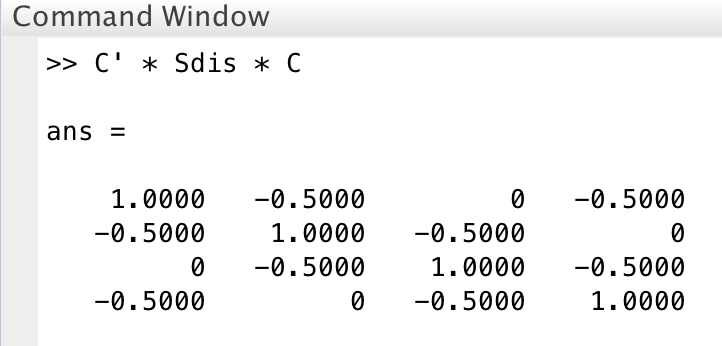
\includegraphics[width=0.5\textwidth]{assets/question_1_matlab.png}
    \caption{MATLAB computation of the global \textbf{S}-matrix}
    \label{fig:q1_matlab}
\end{figure}

\vspace{0.25in}
\begin{center}
\boxed{
	S = 
            \begin{bmatrix}
                1 & -0.5 & 0 & -0.5\\
                -0.5 & 1 & -0.5 & 0\\
                0 & -0.5 & 1 & -0.5\\
                -0.5 & 0 & -0.5 & 1\\
            \end{bmatrix}
}
\end{center}


\end{document}






